\let\negmedspace\undefined
\let\negthickspace\undefined
\documentclass[journal]{IEEEtran}
\usepackage[a5paper, margin=10mm, onecolumn]{geometry}
%\usepackage{lmodern} % Ensure lmodern is loaded for pdflatex
\usepackage{tfrupee} % Include tfrupee package

\setlength{\headheight}{1cm} % Set the height of the header box
\setlength{\headsep}{0mm}     % Set the distance between the header box and the top of the text

\usepackage{gvv-book}
\usepackage{gvv}
\usepackage{cite}
\usepackage{amsmath,amssymb,amsfonts,amsthm}
\usepackage{algorithmic}
\usepackage{graphicx}
\usepackage{textcomp}
\usepackage{xcolor}
\usepackage{txfonts}
\usepackage{listings}
\usepackage{enumitem}
\usepackage{mathtools}
\usepackage{gensymb}
\usepackage{comment}
\usepackage[breaklinks=true]{hyperref}
\usepackage{tkz-euclide} 
\usepackage{listings}
% \usepackage{gvv}                                        
\def\inputGnumericTable{}                                 
\usepackage[latin1]{inputenc}                                
\usepackage{color}                                            
\usepackage{array}                                            
\usepackage{longtable}                                       
\usepackage{calc}                                             
\usepackage{multirow}                                         
\usepackage{hhline}                                           
\usepackage{ifthen}                                           
\usepackage{lscape}
\begin{document}

\bibliographystyle{IEEEtran}
\vspace{3cm}

\title{2.10.57}
\author{EE25btech11028 - J.Navya sri}
% \maketitle
% \newpage
% \bigskip
{\let\newpage\relax\maketitle}


\textbf{Question:} \\
If $\mathbf{a}, \mathbf{b}, \mathbf{c}$ and $\mathbf{d}$ are unit vectors such that 
\[
(\mathbf{a} \times \mathbf{b}) \cdot (\mathbf{c} \times \mathbf{d}) = 1
\quad \text{and} \quad 
\mathbf{a} \cdot \mathbf{c} = \tfrac{1}{2},
\]
then

\begin{enumerate}
    \item[(a)] $\mathbf{a}, \mathbf{b}, \mathbf{c}$ are non-coplanar
    \item[(b)] $\mathbf{b}, \mathbf{c}, \mathbf{d}$ are non-coplanar
    \item[(c)] $\mathbf{b}, \mathbf{d}$ are non-parallel
    \item[(d)] $\mathbf{a}, \mathbf{d}$ are parallel and $\mathbf{b}, \mathbf{c}$ are parallel
\end{enumerate}

\textbf{Soultion:}
We are given that 
\begin{equation}
(\mathbf{a} \times \mathbf{b}) \cdot (\mathbf{c} \times \mathbf{d}) = 1,
\qquad 
\mathbf{a} \cdot \mathbf{c} = \tfrac{1}{2}.
\end{equation}

\textbf{Step 1: Vector Identity}
\begin{equation}
(\mathbf{a} \times \mathbf{b}) \cdot (\mathbf{c} \times \mathbf{d})
= (\mathbf{a} \cdot \mathbf{c})(\mathbf{b} \cdot \mathbf{d}) 
- (\mathbf{a} \cdot \mathbf{d})(\mathbf{b} \cdot \mathbf{c}).
\end{equation}

\textbf{Step 2: Substitution}
Since $\mathbf{a}\cdot \mathbf{c}=\tfrac12$,
\begin{equation}
1 = \tfrac12 (\mathbf{b} \cdot \mathbf{d}) - (\mathbf{a} \cdot \mathbf{d})(\mathbf{b} \cdot \mathbf{c}).
\end{equation}

\textbf{Step 3: Assume $\mathbf{b} \parallel \mathbf{d}$}
If $\mathbf{b} \cdot \mathbf{d} = 1$, then
\begin{equation}
1 = \tfrac12 (1) - (\mathbf{a} \cdot \mathbf{d})(\mathbf{b} \cdot \mathbf{c}).
\end{equation}

\begin{equation}
1 = \tfrac12 - (\mathbf{a} \cdot \mathbf{d})(\mathbf{b} \cdot \mathbf{c}).
\end{equation}

\begin{equation}
(\mathbf{a} \cdot \mathbf{d})(\mathbf{b} \cdot \mathbf{c}) = -\tfrac12.
\end{equation}

\textbf{Step 4: Conclusion}
Thus, the condition is satisfied when
\begin{equation}
\mathbf{a} \parallel \mathbf{d}, 
\qquad 
\mathbf{b} \parallel \mathbf{c}.
\end{equation}

\[
\boxed{\text{Option (D) is correct.}}
\]


\begin{figure}[H]
\begin{center}
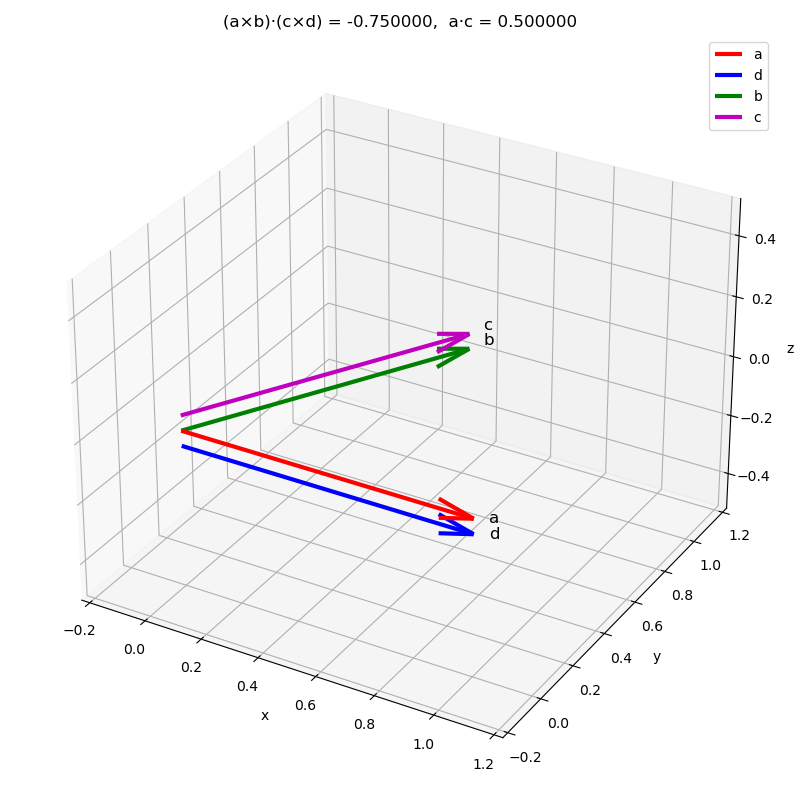
\includegraphics[width=0.6\columnwidth]{figs/fig5.png}
\end{center}
\caption{}
\label{fig:Fig}
\end{figure}


\end{document}